\documentclass[12pt,fleqn]{article}\usepackage{../../common}
\begin{document}
�zkodlama (Autoencoding)

Ozkodlamanin yaptiginin bir tur "veriyi sikistirma" islemi
soylenebilir. Yapay ogrenmede algoritmalarin denetimli ve denetimsiz
olarak ikiye ayrildigindan bahsetmistik, ozkodlama denetimsiz calisir
yani ortada etiket yoktur, daha dogrusu ozkodlama verinin kendisini
etiket olarak kullanir.

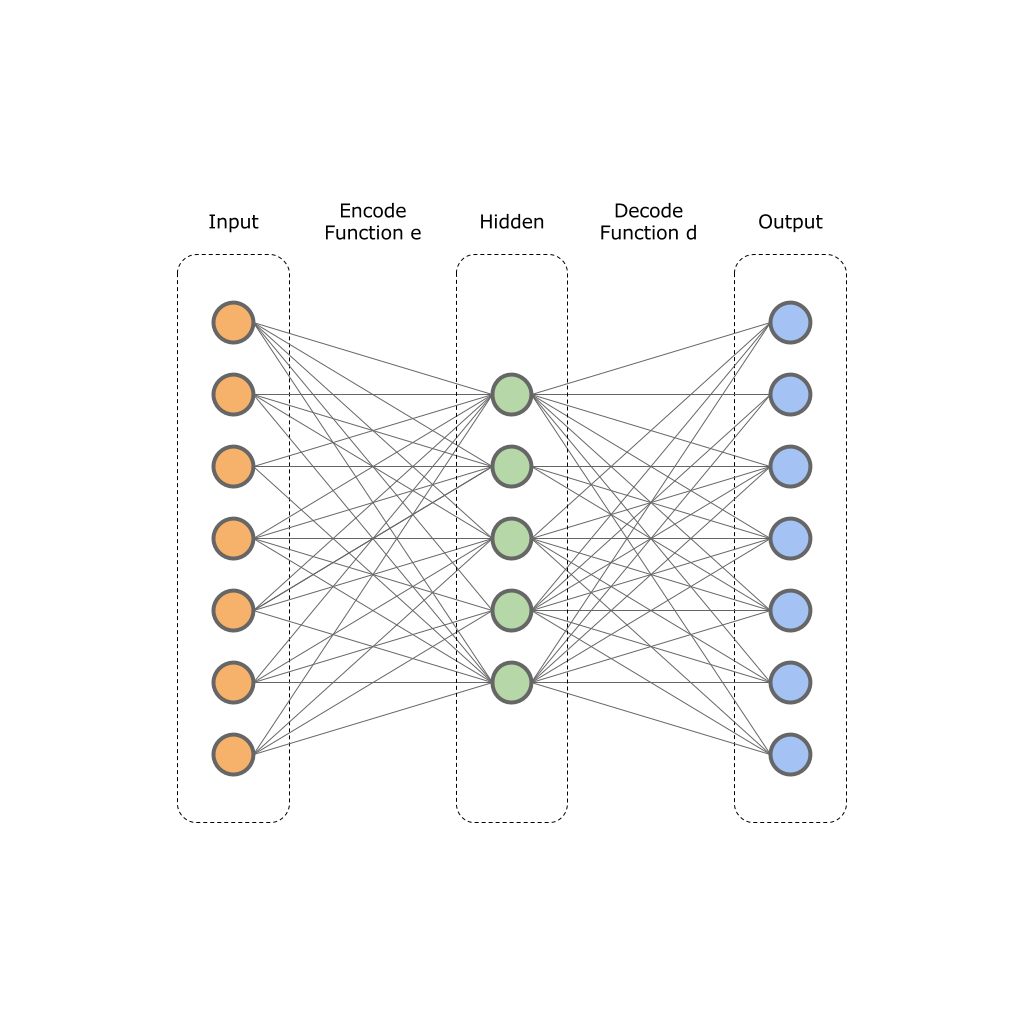
\includegraphics[width=20em]{autoenc_02.png}

Yani girdi olarak verilen veriyi cikti olarak ta kullanirsak, YSA'yi
kendi ciktisini tekrar olusturmayi ogrenmeye zorlamis oluruz, bu
YSA'yi veriyi ozetlemeye dogru yoneltecektir, ve bu tekrar olusturma
icin ileri besleme sirasinda veriyi dar bir noktadan gecmeye zorlarsak
(ustteki resimde goruluyor, 7 noronluk girdi 5 noronluk "daha dar" bir
katmandan gecmeye zorlaniyor), bu YSA'yi "sikistirma" yapmaya daha da
meyillendirecektir.

\begin{minted}[fontsize=\footnotesize]{python}
from keras.datasets import mnist
import mnist_autoenc

(x_train, _), (x_test, _) = mnist.load_data()
x_test = x_test.astype('float32') / 255.
autoencoder, encoder, decoder = mnist_autoenc.get_model()
encoder.load_weights("mod-enc-1.h5")
decoder.load_weights("mod-dec-1.h5")
\end{minted}

\begin{minted}[fontsize=\footnotesize]{python}
tmp = x_test[1090, :, :].reshape(1,28*28)
encoded = encoder.predict(tmp)
print (encoded.shape)
decoded = decoder.predict(encoded).reshape(28,28)
print (decoded.shape)
plt.imshow(decoded)
plt.gray()
plt.savefig('autoenc_01.png')
\end{minted}

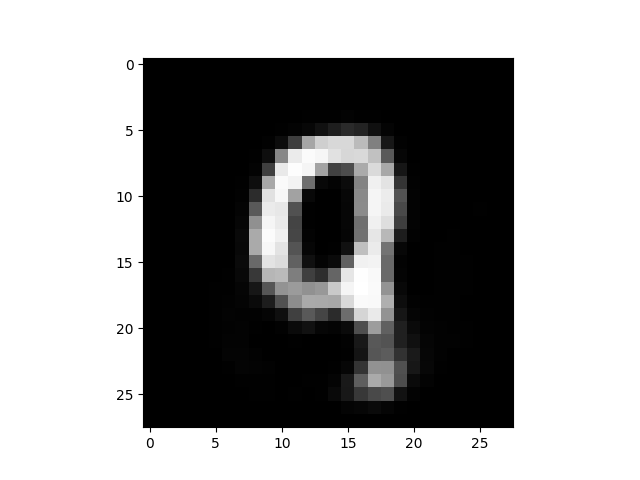
\includegraphics[width=20em]{autoenc_01.png}

\begin{minted}[fontsize=\footnotesize]{python}
import mnist_autoenc_rnn_simple

seq_autoencoder, encoder = mnist_autoenc_rnn_simple.get_model()
seq_autoencoder.load_weights("mod-rnn-autoenc-sim.h5")
encoder.load_weights("mod-rnn-enc-sim.h5")
\end{minted}

\begin{minted}[fontsize=\footnotesize]{python}
decoded = seq_autoencoder.predict(tmp).reshape(28,28)
print (decoded.shape)
plt.imshow(decoded)
plt.gray()
plt.savefig('autoenc_03.png')
\end{minted}

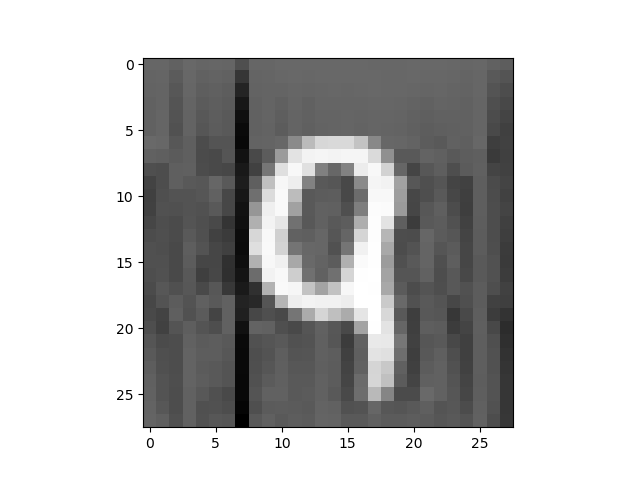
\includegraphics[width=20em]{autoenc_03.png}

Varyasyonel Ozkodlayicilar

Standard ozkodlayicilarin bir problemi kodlama yaptiklari daralmis
alandaki vektorlerin surekli olmayabilecegi, ve buradaki degerlerin
kolay bir sekilde interpolasyon yapilmasindaki bazi zorluklar.

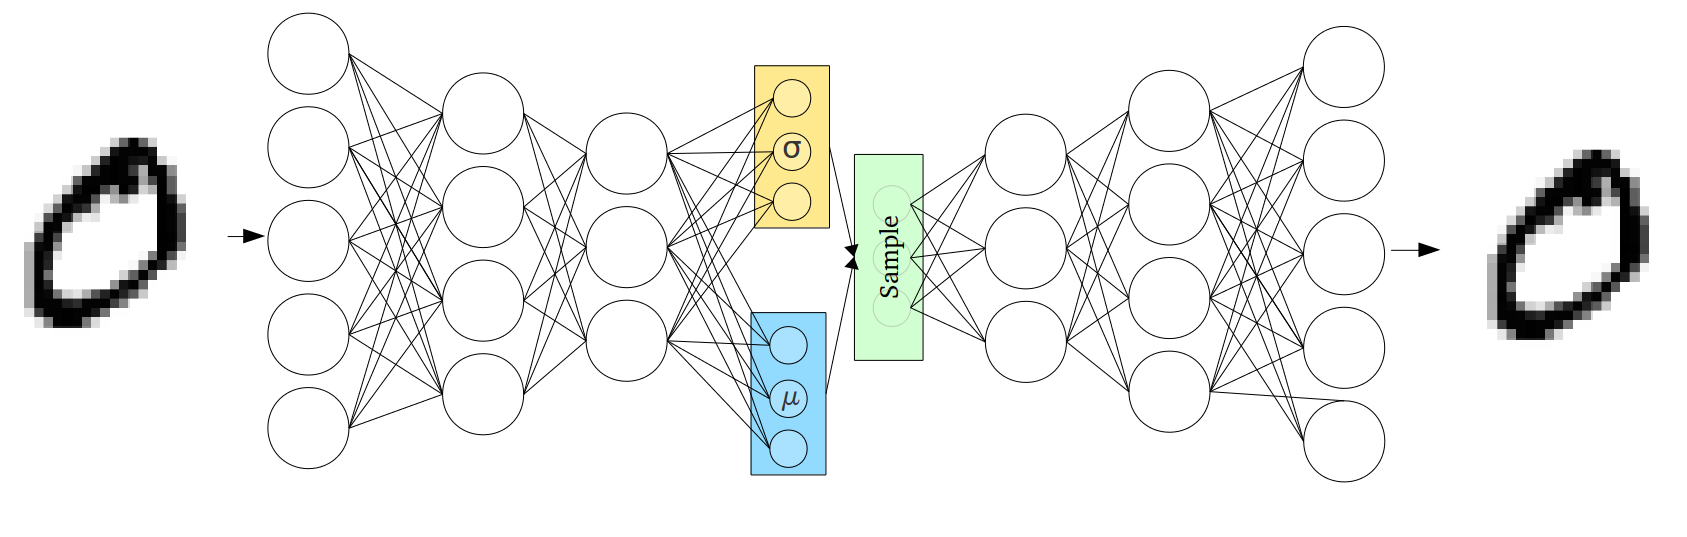
\includegraphics[width=20em]{autoenc_06.png}

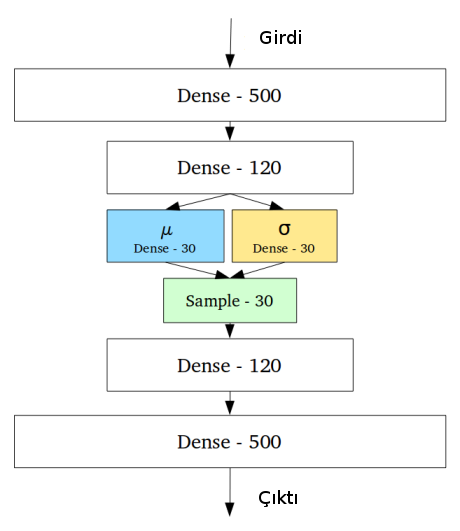
\includegraphics[width=20em]{autoenc_07.png}

\begin{minted}[fontsize=\footnotesize]{python}
import mnist_lstm_vae

vae, enc, gen = mnist_lstm_vae.create_lstm_vae(mnist_lstm_vae.input_dim, 
    timesteps=mnist_lstm_vae.timesteps, 
    batch_size=mnist_lstm_vae.batch_size, 
    intermediate_dim=mnist_lstm_vae.latent_dim,
    latent_dim=mnist_lstm_vae.latent_dim,
    epsilon_std=1.)
vae.load_weights('mnist_lstm_vae.h5')
enc.load_weights('mnist_lstm_enc.h5')
\end{minted}

\begin{minted}[fontsize=\footnotesize]{python}
import random
idx = 400
print (tmp.shape)
x_test_tmp = x_test[idx]
res = vae.predict(x_test_tmp.reshape((1, 28, 28)))

plt.figure()
ax = plt.subplot(1, 2, 1)
pixels = res.reshape((28, 28))
plt.imshow(pixels)
plt.gray()
ax = plt.subplot(1, 2, 2)
plt.imshow(x_test_tmp)
plt.gray()

plt.savefig('autoenc_04.png')
\end{minted}

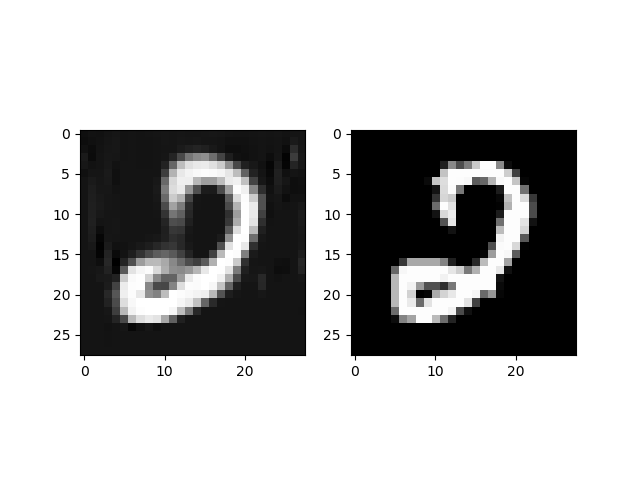
\includegraphics[width=20em]{autoenc_04.png}

\begin{minted}[fontsize=\footnotesize]{python}
import aae_normal
latent_dim = 100
input_shape = (28, 28)
encoder = aae_normal.model_encoder(latent_dim, input_shape)
encoder.load_weights('aae-norm-encoder.h5')
generator = aae_normal.model_generator(latent_dim, input_shape)
generator.load_weights('aae-norm-generator.h5')
\end{minted}

\begin{minted}[fontsize=\footnotesize]{python}
idx = 100
print (x_test[idx, :].shape)
res = encoder.predict(x_test[idx, :].reshape(1,28,28))
print (res.shape)
pixels = generator.predict(res)
pixels = pixels.reshape((28, 28))
plt.imshow(pixels)
plt.gray()
plt.savefig('autoenc_05.png')
\end{minted}

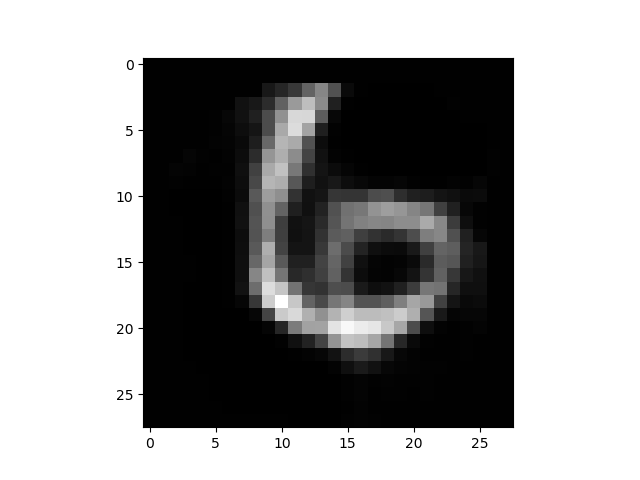
\includegraphics[width=20em]{autoenc_05.png}



Kaynaklar

[1] \url{https://blog.keras.io/building-autoencoders-in-keras.html}

[2] adverserial autoencoder keras \url{https://github.com/bstriner/keras-adversarial/blob/master/examples/example_aae.py}

[3] \url{https://towardsdatascience.com/intuitively-understanding-variational-autoencoders-1bfe67eb5daf}

[4] \url{https://hsaghir.github.io/data_science/denoising-vs-variational-autoencoder/}

[5] Doersch, Tutorial on Variational Autoencoders, \url{https://arxiv.org/pdf/1606.05908.pdf}

[6] Goodfellow, Adversarial Autoencoders, \url{https://arxiv.org/pdf/1511.05644.pdf}

[7] What is Adversarial Autoencoder?, \url{https://www.quora.com/What-is-Adversarial-Autoencoder}

[8] \url{http://www.inference.vc/adversarial-autoencoders/}


\end{document}
